\documentclass[tikz,border=2pt]{standalone}
\usepackage{amsmath}
\usetikzlibrary{arrows.meta}
% \cells{x0}{y0}{cols}{rows}{colour}: draw a cols x rows grid with top-left corner (x0,y0)
\newcommand{\cells}[5]{%
  \foreach \i in {0,...,#3} \draw[#5] ({#1+\i},#2) -- ({#1+\i},{#2-#4});%
  \foreach \j in {0,...,#4} \draw[#5] (#1,{#2-\j}) -- ({#1+#3},{#2-\j});%
  \draw[#5, thick] (#1,#2) rectangle ({#1+#3},{#2-#4});}
\begin{document}
% Top: A %*% B for a 2x3 and a 3x2 matrix gives 2x2; row 1 of A and column 2 of B fill entry (1,2).
% Bottom: A * C for two 2x3 matrices multiplies entries in the same position and keeps the shape 2x3.
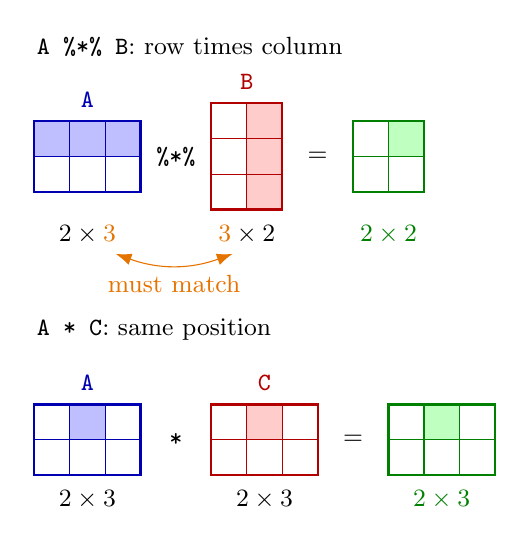
\begin{tikzpicture}[font=\small, >={Latex[length=2mm]}, x=0.45cm, y=0.45cm]
  % ---------- matrix product ----------
  \node[anchor=west] at (-0.2,2.1) {\texttt{A \%*\% B}: row times column};
  % A: 2 x 3
  \fill[blue!25] (0,0) rectangle (3,-1);
  \cells{0}{0}{3}{2}{blue!70!black}
  \node[blue!70!black] at (1.5,0.6) {\texttt{A}};
  \node at (4,-1) {\texttt{\%*\%}};
  % B: 3 x 2
  \fill[red!20] (6,0.5) rectangle (7,-2.5);
  \cells{5}{0.5}{2}{3}{red!70!black}
  \node[red!70!black] at (6,1.1) {\texttt{B}};
  \node at (8,-1) {$=$};
  % result: 2 x 2
  \fill[green!25] (10,0) rectangle (11,-1);
  \cells{9}{0}{2}{2}{green!50!black}
  % dimension labels
  \node at (1.5,-3.2) {$2\times\textcolor{orange!90!black}{3}$};
  \node at (6,-3.2) {$\textcolor{orange!90!black}{3}\times2$};
  \node[green!50!black] at (10,-3.2) {$2\times2$};
  \draw[orange!90!black, <->] (2.3,-3.75) to[bend right=20] node[below] {must match} (5.6,-3.75);
  % ---------- entrywise product ----------
  \begin{scope}[yshift=-3.6cm]
  \node[anchor=west] at (-0.2,2.1) {\texttt{A * C}: same position};
  \fill[blue!25] (1,0) rectangle (2,-1);
  \cells{0}{0}{3}{2}{blue!70!black}
  \node[blue!70!black] at (1.5,0.6) {\texttt{A}};
  \node at (4,-1) {\texttt{*}};
  \fill[red!20] (6,0) rectangle (7,-1);
  \cells{5}{0}{3}{2}{red!70!black}
  \node[red!70!black] at (6.5,0.6) {\texttt{C}};
  \node at (9,-1) {$=$};
  \fill[green!25] (11,0) rectangle (12,-1);
  \cells{10}{0}{3}{2}{green!50!black}
  \node at (1.5,-2.7) {$2\times3$};
  \node at (6.5,-2.7) {$2\times3$};
  \node[green!50!black] at (11.5,-2.7) {$2\times3$};
  \end{scope}
\end{tikzpicture}
\end{document}
